\documentclass[]{tufte-handout}

% ams
\usepackage{amssymb,amsmath}

\usepackage{ifxetex,ifluatex}
\usepackage{fixltx2e} % provides \textsubscript
\ifnum 0\ifxetex 1\fi\ifluatex 1\fi=0 % if pdftex
  \usepackage[T1]{fontenc}
  \usepackage[utf8]{inputenc}
\else % if luatex or xelatex
  \makeatletter
  \@ifpackageloaded{fontspec}{}{\usepackage{fontspec}}
  \makeatother
  \defaultfontfeatures{Ligatures=TeX,Scale=MatchLowercase}
  \makeatletter
  \@ifpackageloaded{soul}{
     \renewcommand\allcapsspacing[1]{{\addfontfeature{LetterSpace=15}#1}}
     \renewcommand\smallcapsspacing[1]{{\addfontfeature{LetterSpace=10}#1}}
   }{}
  \makeatother

\fi

% graphix
\usepackage{graphicx}
\setkeys{Gin}{width=\linewidth,totalheight=\textheight,keepaspectratio}

% booktabs
\usepackage{booktabs}

% url
\usepackage{url}

% hyperref
\usepackage{hyperref}

% units.
\usepackage{units}


\setcounter{secnumdepth}{-1}

% citations
\usepackage{natbib}
\bibliographystyle{plainnat}


% pandoc syntax highlighting
\usepackage{color}
\usepackage{fancyvrb}
\newcommand{\VerbBar}{|}
\newcommand{\VERB}{\Verb[commandchars=\\\{\}]}
\DefineVerbatimEnvironment{Highlighting}{Verbatim}{commandchars=\\\{\}}
% Add ',fontsize=\small' for more characters per line
\newenvironment{Shaded}{}{}
\newcommand{\AlertTok}[1]{\textcolor[rgb]{1.00,0.00,0.00}{\textbf{#1}}}
\newcommand{\AnnotationTok}[1]{\textcolor[rgb]{0.38,0.63,0.69}{\textbf{\textit{#1}}}}
\newcommand{\AttributeTok}[1]{\textcolor[rgb]{0.49,0.56,0.16}{#1}}
\newcommand{\BaseNTok}[1]{\textcolor[rgb]{0.25,0.63,0.44}{#1}}
\newcommand{\BuiltInTok}[1]{\textcolor[rgb]{0.00,0.50,0.00}{#1}}
\newcommand{\CharTok}[1]{\textcolor[rgb]{0.25,0.44,0.63}{#1}}
\newcommand{\CommentTok}[1]{\textcolor[rgb]{0.38,0.63,0.69}{\textit{#1}}}
\newcommand{\CommentVarTok}[1]{\textcolor[rgb]{0.38,0.63,0.69}{\textbf{\textit{#1}}}}
\newcommand{\ConstantTok}[1]{\textcolor[rgb]{0.53,0.00,0.00}{#1}}
\newcommand{\ControlFlowTok}[1]{\textcolor[rgb]{0.00,0.44,0.13}{\textbf{#1}}}
\newcommand{\DataTypeTok}[1]{\textcolor[rgb]{0.56,0.13,0.00}{#1}}
\newcommand{\DecValTok}[1]{\textcolor[rgb]{0.25,0.63,0.44}{#1}}
\newcommand{\DocumentationTok}[1]{\textcolor[rgb]{0.73,0.13,0.13}{\textit{#1}}}
\newcommand{\ErrorTok}[1]{\textcolor[rgb]{1.00,0.00,0.00}{\textbf{#1}}}
\newcommand{\ExtensionTok}[1]{#1}
\newcommand{\FloatTok}[1]{\textcolor[rgb]{0.25,0.63,0.44}{#1}}
\newcommand{\FunctionTok}[1]{\textcolor[rgb]{0.02,0.16,0.49}{#1}}
\newcommand{\ImportTok}[1]{\textcolor[rgb]{0.00,0.50,0.00}{\textbf{#1}}}
\newcommand{\InformationTok}[1]{\textcolor[rgb]{0.38,0.63,0.69}{\textbf{\textit{#1}}}}
\newcommand{\KeywordTok}[1]{\textcolor[rgb]{0.00,0.44,0.13}{\textbf{#1}}}
\newcommand{\NormalTok}[1]{#1}
\newcommand{\OperatorTok}[1]{\textcolor[rgb]{0.40,0.40,0.40}{#1}}
\newcommand{\OtherTok}[1]{\textcolor[rgb]{0.00,0.44,0.13}{#1}}
\newcommand{\PreprocessorTok}[1]{\textcolor[rgb]{0.74,0.48,0.00}{#1}}
\newcommand{\RegionMarkerTok}[1]{#1}
\newcommand{\SpecialCharTok}[1]{\textcolor[rgb]{0.25,0.44,0.63}{#1}}
\newcommand{\SpecialStringTok}[1]{\textcolor[rgb]{0.73,0.40,0.53}{#1}}
\newcommand{\StringTok}[1]{\textcolor[rgb]{0.25,0.44,0.63}{#1}}
\newcommand{\VariableTok}[1]{\textcolor[rgb]{0.10,0.09,0.49}{#1}}
\newcommand{\VerbatimStringTok}[1]{\textcolor[rgb]{0.25,0.44,0.63}{#1}}
\newcommand{\WarningTok}[1]{\textcolor[rgb]{0.38,0.63,0.69}{\textbf{\textit{#1}}}}

% table with pandoc

% multiplecol
\usepackage{multicol}

% strikeout
\usepackage[normalem]{ulem}

% morefloats
\usepackage{morefloats}


% tightlist macro required by pandoc >= 1.14
\providecommand{\tightlist}{%
  \setlength{\itemsep}{0pt}\setlength{\parskip}{0pt}}

% title / author / date
\title[Using the fastQR package]{Using the fastQR package}
\author{Mauro Bernardi}
\date{2025-01-28}


\begin{document}

\maketitle




\hypertarget{introduction}{%
\section{Introduction}\label{introduction}}

In numerical linear algebra, matrix factorization techniques are
fundamental for solving systems of equations, least squares problems,
and eigenvalue computations. One of the most widely used methods is the
QR decomposition, which factors a given matrix
\(A \in \mathbb{R}^{m \times n}\) into the product of an orthogonal
matrix \(Q\) and an upper triangular matrix \(R\). The decomposition is
particularly advantageous due to its numerical stability and efficiency
when applied to various computational problems, including solving linear
systems and computing the singular value decomposition (SVD)
\cite{golub2013matrix}.

QR decomposition can be computed through several algorithms, such as the
Gram-Schmidt process, Householder reflections, and Givens rotations,
each offering different trade-offs in terms of computational efficiency
and numerical stability. The Gram-Schmidt process provides an intuitive
geometrical approach but may suffer from numerical instability,
especially in the presence of nearly linearly dependent columns. On the
other hand, Householder reflections are more numerically stable and
computationally efficient for large matrices. Givens rotations are
particularly suited for sparse matrices due to their ability to zero out
specific elements in the matrix.

Due to its versatility and importance in both theoretical and practical
contexts, QR decomposition has been extensively studied and remains a
fundamental tool in scientific computing and data analysis.

We introduce two innovative R packages, designed for high-performance
statistical computing (\texttt{C++ Eigen}):

\begin{enumerate}
\def\labelenumi{\arabic{enumi}.}
\tightlist
\item
  \texttt{fastQR}: a package for efficient QR decomposition,
  updating/downdating. It enhances QR decomposition processes, including
  updates and downdates of the QR, R and L decompositions;
\item
  \texttt{fastBVS}: a tool for Bayesian variable selection. It provides
  advanced techniques that enables flexible and efficient model
  selection in Bayesian frameworks. \uline{Key} features are:
\end{enumerate}

\begin{itemize}
\tightlist
\item
  RJ-type algorithms, with Dirac spike-and-slab (DSS) prior;
\item
  consider both linear Gaussian and probit regressions;
\item
  consider both univariate and multivariate responses;
\item
  SSVS algorithms, with DSS and continuous spike-and-slab (CSS) prior;
\item
  tools for fast processing and analyzing the output, monitoring
  convergence, hyper-parameters CV, \ldots
\end{itemize}

\hypertarget{computational-time}{%
\section{Computational time}\label{computational-time}}

Compuational time for the QR factorization of the matrix
\(\bX\in\mathbb{R}^{n\times p}\), with \(n=2000\) fixed, see Golub \&
van Loan (2013).

\begin{Shaded}
\begin{Highlighting}[]
\FunctionTok{library}\NormalTok{(rbenchmark)}
\FunctionTok{library}\NormalTok{(fastQR)}
\end{Highlighting}
\end{Shaded}

\begin{verbatim}
## 
## Attaching package: 'fastQR'
\end{verbatim}

\begin{verbatim}
## The following object is masked from 'package:base':
## 
##     qr
\end{verbatim}

\begin{Shaded}
\begin{Highlighting}[]
\DocumentationTok{\#\# generate sample data}
\FunctionTok{set.seed}\NormalTok{(}\DecValTok{1234}\NormalTok{)}
\NormalTok{n }\OtherTok{\textless{}{-}} \DecValTok{1000}
\NormalTok{p }\OtherTok{\textless{}{-}} \DecValTok{500}
\NormalTok{X }\OtherTok{\textless{}{-}} \FunctionTok{matrix}\NormalTok{(}\FunctionTok{rnorm}\NormalTok{(n }\SpecialCharTok{*}\NormalTok{ p, }\DecValTok{1}\NormalTok{), n, p)}

\DocumentationTok{\#\# QR decomposition}
\FunctionTok{benchmark}\NormalTok{(}\StringTok{"fastQR"} \OtherTok{=}\NormalTok{ fastQR}\SpecialCharTok{::}\FunctionTok{qr}\NormalTok{(X, }\AttributeTok{nb =} \DecValTok{5}\NormalTok{),}
          \StringTok{"R base"} \OtherTok{=}\NormalTok{ base}\SpecialCharTok{::}\FunctionTok{qr}\NormalTok{(X),}
          \AttributeTok{replications =} \DecValTok{100}\NormalTok{,}
          \AttributeTok{columns =} \FunctionTok{c}\NormalTok{(}\StringTok{"test"}\NormalTok{, }\StringTok{"replications"}\NormalTok{, }\StringTok{"elapsed"}\NormalTok{,}
                      \StringTok{"relative"}\NormalTok{, }\StringTok{"user.self"}\NormalTok{, }\StringTok{"sys.self"}\NormalTok{))}
\end{Highlighting}
\end{Shaded}

\begin{verbatim}
##     test replications elapsed relative user.self sys.self
## 1 fastQR          100   2.392    1.000     2.251    0.135
## 2 R base          100  11.747    4.911    11.688    0.042
\end{verbatim}

\hypertarget{qr-decomposition}{%
\section{QR decomposition}\label{qr-decomposition}}

\begin{Shaded}
\begin{Highlighting}[]
\FunctionTok{load}\NormalTok{(}\StringTok{"QRfact\_boxplot.RData"}\NormalTok{)}
\FunctionTok{print}\NormalTok{(output }\SpecialCharTok{\%\textgreater{}\%}
        \FunctionTok{group\_by}\NormalTok{(p, method) }\SpecialCharTok{\%\textgreater{}\%}
        \FunctionTok{get\_summary\_stats}\NormalTok{(), }\AttributeTok{n =} \DecValTok{12}\NormalTok{)}
\end{Highlighting}
\end{Shaded}

\begin{verbatim}
## # A tibble: 27 x 15
##        p method  variable     n   min   max median    q1    q3   iqr   mad  mean
##    <dbl> <chr>   <fct>    <dbl> <dbl> <dbl>  <dbl> <dbl> <dbl> <dbl> <dbl> <dbl>
##  1    20 baseQR  time        20 0     0.001  0.001 0.001 0.001 0     0     0.001
##  2    20 rb QR,~ time        20 0.001 0.009  0.002 0.002 0.002 0     0     0.002
##  3    20 rb QR,~ time        20 0     0.003  0.001 0.001 0.002 0.001 0.001 0.002
##  4    40 baseQR  time        20 0.002 0.005  0.003 0.003 0.004 0.001 0.001 0.003
##  5    40 rb QR,~ time        20 0.003 0.008  0.005 0.005 0.006 0.001 0.001 0.005
##  6    40 rb QR,~ time        20 0.002 0.004  0.003 0.003 0.003 0     0     0.003
##  7   100 baseQR  time        20 0.012 0.019  0.014 0.013 0.016 0.003 0.002 0.015
##  8   100 rb QR,~ time        20 0.006 0.019  0.012 0.011 0.014 0.003 0.002 0.012
##  9   100 rb QR,~ time        20 0.006 0.017  0.01  0.009 0.012 0.003 0.003 0.01 
## 10   200 baseQR  time        20 0.051 0.072  0.06  0.055 0.063 0.009 0.007 0.06 
## 11   200 rb QR,~ time        20 0.021 0.05   0.041 0.031 0.043 0.012 0.006 0.038
## 12   200 rb QR,~ time        20 0.019 0.036  0.026 0.024 0.029 0.005 0.004 0.027
## # i 15 more rows
## # i 3 more variables: sd <dbl>, se <dbl>, ci <dbl>
\end{verbatim}

\begin{Shaded}
\begin{Highlighting}[]
\CommentTok{\# Convert factors to appropriate types}
\NormalTok{output}\SpecialCharTok{$}\NormalTok{p }\OtherTok{\textless{}{-}} \FunctionTok{as.factor}\NormalTok{(output}\SpecialCharTok{$}\NormalTok{p)}

\CommentTok{\# Plot the results}
\NormalTok{boxplot }\OtherTok{\textless{}{-}} \FunctionTok{ggplot}\NormalTok{(output, }\FunctionTok{aes}\NormalTok{(}\AttributeTok{x =}\NormalTok{ p, }\AttributeTok{y =}\NormalTok{ time)) }\SpecialCharTok{+}
  \FunctionTok{geom\_boxplot}\NormalTok{(}\FunctionTok{aes}\NormalTok{(}\AttributeTok{color =}\NormalTok{ method)) }\SpecialCharTok{+}
  \FunctionTok{labs}\NormalTok{(}
    \AttributeTok{x =} \StringTok{"p"}\NormalTok{,}
    \AttributeTok{y =} \StringTok{"time (seconds)"}\NormalTok{,}
    \AttributeTok{fill =} \StringTok{"method"}
\NormalTok{  ) }\SpecialCharTok{+}
  \FunctionTok{theme\_classic}\NormalTok{() }\SpecialCharTok{+}  
  \FunctionTok{theme}\NormalTok{(}\AttributeTok{text =} \FunctionTok{element\_text}\NormalTok{(}\AttributeTok{size =} \DecValTok{22}\NormalTok{)) }\SpecialCharTok{+}
  \FunctionTok{theme}\NormalTok{(}\AttributeTok{axis.text.x =} \FunctionTok{element\_text}\NormalTok{(}\AttributeTok{angle =} \DecValTok{0}\NormalTok{, }\AttributeTok{vjust =} \FloatTok{0.0}\NormalTok{, }\AttributeTok{hjust =}\NormalTok{ .}\DecValTok{50}\NormalTok{)) }\SpecialCharTok{+}
  \FunctionTok{theme}\NormalTok{(}
    \AttributeTok{legend.background    =} \FunctionTok{element\_rect}\NormalTok{(}\AttributeTok{fill =} \StringTok{"white"}\NormalTok{, }\AttributeTok{linewidth =} \DecValTok{4}\NormalTok{, }\AttributeTok{colour =} \StringTok{"white"}\NormalTok{),}
    \AttributeTok{legend.justification =} \StringTok{"center"}\NormalTok{,}
    \AttributeTok{legend.position      =} \StringTok{"bottom"}
\NormalTok{  ) }\SpecialCharTok{+}
  \CommentTok{\#ylim(c(0, 0.01)) +}
  \FunctionTok{scale\_color\_manual}\NormalTok{(}\AttributeTok{labels =} \FunctionTok{c}\NormalTok{(}\StringTok{"base QR"}\NormalTok{, }\StringTok{"rb QR, nb = 5"}\NormalTok{, }\StringTok{"rb QR, nb = p/2"}\NormalTok{), }\AttributeTok{values =}\NormalTok{ col\_pal) }\SpecialCharTok{+}
  \FunctionTok{guides}\NormalTok{(}\AttributeTok{fill =} \FunctionTok{guide\_legend}\NormalTok{(}\StringTok{"Method"}\NormalTok{)) }

\CommentTok{\# Display the boxplot}
\FunctionTok{print}\NormalTok{(boxplot)}
\end{Highlighting}
\end{Shaded}

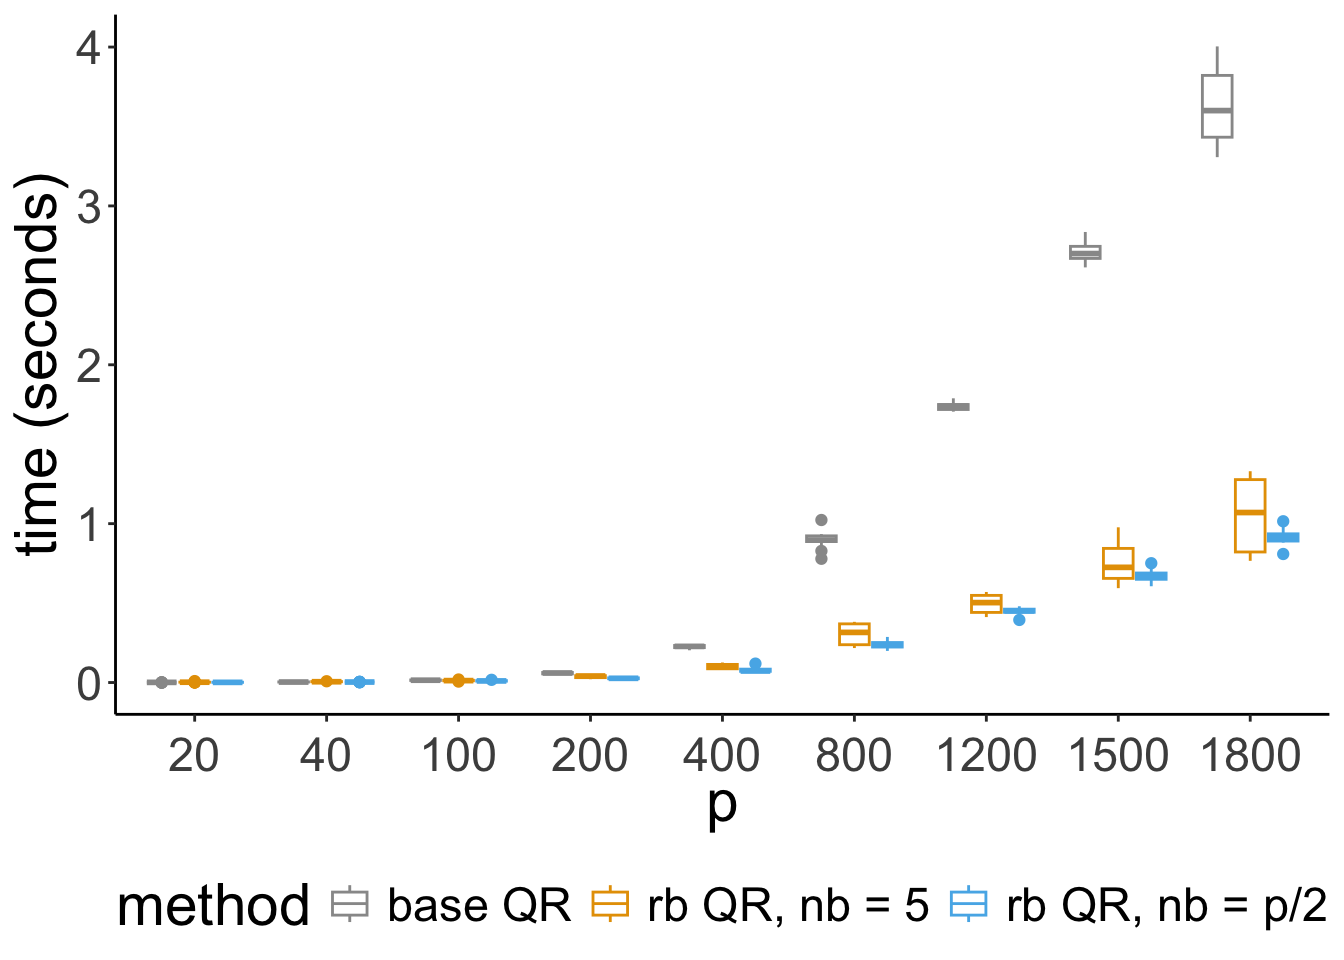
\includegraphics{fastQR_examples_files/figure-latex/unnamed-chunk-4-1}

\hypertarget{cholesky-factorization-via-qr}{%
\section{Cholesky factorization via
QR}\label{cholesky-factorization-via-qr}}

\begin{Shaded}
\begin{Highlighting}[]
\CommentTok{\# Matrix dimensions to test}
\NormalTok{nrep }\OtherTok{\textless{}{-}} \DecValTok{10}
\NormalTok{n    }\OtherTok{\textless{}{-}} \DecValTok{2000}
\NormalTok{p    }\OtherTok{\textless{}{-}} \FunctionTok{c}\NormalTok{(}\DecValTok{20}\NormalTok{, }\DecValTok{40}\NormalTok{, }\DecValTok{100}\NormalTok{, }\DecValTok{200}\NormalTok{, }\DecValTok{400}\NormalTok{, }\DecValTok{800}\NormalTok{, }\DecValTok{1200}\NormalTok{, }\DecValTok{1500}\NormalTok{, }\DecValTok{1800}\NormalTok{)}
\NormalTok{p    }\OtherTok{\textless{}{-}} \FunctionTok{c}\NormalTok{(}\DecValTok{20}\NormalTok{, }\DecValTok{40}\NormalTok{, }\DecValTok{100}\NormalTok{, }\DecValTok{200}\NormalTok{, }\DecValTok{400}\NormalTok{)}

\NormalTok{nrep }\OtherTok{\textless{}{-}} \DecValTok{10}
\NormalTok{n    }\OtherTok{\textless{}{-}} \DecValTok{200}
\NormalTok{p    }\OtherTok{\textless{}{-}} \FunctionTok{c}\NormalTok{(}\DecValTok{20}\NormalTok{, }\DecValTok{40}\NormalTok{, }\DecValTok{60}\NormalTok{, }\DecValTok{80}\NormalTok{, }\DecValTok{100}\NormalTok{, }\DecValTok{120}\NormalTok{, }\DecValTok{140}\NormalTok{, }\DecValTok{160}\NormalTok{, }\DecValTok{180}\NormalTok{)}
\NormalTok{p}\SpecialCharTok{/}\DecValTok{4}

\FunctionTok{detectCores}\NormalTok{()}
\NormalTok{ncores }\OtherTok{\textless{}{-}} \DecValTok{10}
\FunctionTok{registerDoParallel}\NormalTok{(}\AttributeTok{cores =}\NormalTok{ ncores)}

\CommentTok{\# Benchmark QR and Cholesky decomposition for each dimension}
\NormalTok{output  }\OtherTok{\textless{}{-}} \ConstantTok{NULL}
\FunctionTok{set.seed}\NormalTok{(}\DecValTok{1234}\NormalTok{)}
\ControlFlowTok{for}\NormalTok{ (dim }\ControlFlowTok{in}\NormalTok{ p) \{}
\NormalTok{  results }\OtherTok{\textless{}{-}} \ConstantTok{NULL}
\NormalTok{  results }\OtherTok{\textless{}{-}}\NormalTok{ foreach}\SpecialCharTok{::}\FunctionTok{foreach}\NormalTok{(}\AttributeTok{rep =} \DecValTok{1}\SpecialCharTok{:}\NormalTok{nrep, }\AttributeTok{.packages =} \FunctionTok{c}\NormalTok{(}\StringTok{"fastQR"}\NormalTok{), }\AttributeTok{.combine =} \StringTok{"rbind"}\NormalTok{) }\SpecialCharTok{\%dopar\%}\NormalTok{ \{}
    \CommentTok{\#for (rep in 1:nrep) \{ }
    \CommentTok{\# print}
    \FunctionTok{cat}\NormalTok{(}\StringTok{"rep "}\NormalTok{, rep, }\StringTok{"}\SpecialCharTok{\textbackslash{}n}\StringTok{"}\NormalTok{)}
    
    \CommentTok{\# set seed}
    \CommentTok{\#set.seed(1234 + rep)}
    
    \CommentTok{\# Generate a random matrix}
\NormalTok{    mat  }\OtherTok{\textless{}{-}} \FunctionTok{matrix}\NormalTok{(}\FunctionTok{rnorm}\NormalTok{(n }\SpecialCharTok{*}\NormalTok{ dim), }\AttributeTok{nrow =}\NormalTok{ n, }\AttributeTok{ncol =}\NormalTok{ dim)}
\NormalTok{    mat2 }\OtherTok{\textless{}{-}} \FunctionTok{crossprod}\NormalTok{(mat)}
    
    \CommentTok{\# Measure fastQR, qr time}
\NormalTok{    qr\_time }\OtherTok{\textless{}{-}} \FunctionTok{system.time}\NormalTok{(fastQR}\SpecialCharTok{::}\FunctionTok{qrchol}\NormalTok{(mat, }\AttributeTok{nb =} \DecValTok{5}\NormalTok{))[}\StringTok{"elapsed"}\NormalTok{]}
\NormalTok{    res1    }\OtherTok{\textless{}{-}} \FunctionTok{data.frame}\NormalTok{(}\AttributeTok{p =}\NormalTok{ dim, }\AttributeTok{method =} \StringTok{"rb QR, nb = 5"}\NormalTok{, }\AttributeTok{time =}\NormalTok{ qr\_time)}
    
\NormalTok{    rbqr\_time }\OtherTok{\textless{}{-}} \FunctionTok{system.time}\NormalTok{(fastQR}\SpecialCharTok{::}\FunctionTok{qrchol}\NormalTok{(}\AttributeTok{X =}\NormalTok{ mat, }\AttributeTok{nb =}\NormalTok{ dim}\SpecialCharTok{/}\DecValTok{2}\NormalTok{))[}\StringTok{"elapsed"}\NormalTok{]}
\NormalTok{    res2      }\OtherTok{\textless{}{-}} \FunctionTok{data.frame}\NormalTok{(}\AttributeTok{p =}\NormalTok{ dim, }\AttributeTok{method =} \StringTok{"rb QR, nb = p/2"}\NormalTok{, }\AttributeTok{time =}\NormalTok{ rbqr\_time)}
    
    \CommentTok{\# Measure Cholesky time}
\NormalTok{    baseqr\_time }\OtherTok{\textless{}{-}} \FunctionTok{system.time}\NormalTok{(base}\SpecialCharTok{::}\FunctionTok{chol}\NormalTok{(mat2))[}\StringTok{"elapsed"}\NormalTok{]}
\NormalTok{    res3        }\OtherTok{\textless{}{-}} \FunctionTok{data.frame}\NormalTok{(}\AttributeTok{p =}\NormalTok{ dim, }\AttributeTok{method =} \StringTok{"baseQR"}\NormalTok{,  }\AttributeTok{time =}\NormalTok{ baseqr\_time)}
    
    \CommentTok{\# return}
    \FunctionTok{rbind}\NormalTok{(results, }\FunctionTok{rbind}\NormalTok{(res1, res2, res3))}
\NormalTok{  \}}
\NormalTok{  output }\OtherTok{\textless{}{-}} \FunctionTok{rbind}\NormalTok{(output, results)}
\NormalTok{\}}
\FunctionTok{save}\NormalTok{(}\AttributeTok{file =} \StringTok{"cholesky\_boxplot.RData"}\NormalTok{, output)}
\end{Highlighting}
\end{Shaded}

\begin{Shaded}
\begin{Highlighting}[]
\FunctionTok{print}\NormalTok{(output }\SpecialCharTok{\%\textgreater{}\%}
        \FunctionTok{group\_by}\NormalTok{(p, method) }\SpecialCharTok{\%\textgreater{}\%}
        \FunctionTok{get\_summary\_stats}\NormalTok{(), }\AttributeTok{n =} \DecValTok{27}\NormalTok{)}
\end{Highlighting}
\end{Shaded}

\begin{verbatim}
## # A tibble: 27 x 15
##    p     method  variable     n   min   max median    q1    q3   iqr   mad  mean
##    <fct> <chr>   <fct>    <dbl> <dbl> <dbl>  <dbl> <dbl> <dbl> <dbl> <dbl> <dbl>
##  1 20    baseQR  time        20 0     0.001  0.001 0.001 0.001 0     0     0.001
##  2 20    rb QR,~ time        20 0.001 0.009  0.002 0.002 0.002 0     0     0.002
##  3 20    rb QR,~ time        20 0     0.003  0.001 0.001 0.002 0.001 0.001 0.002
##  4 40    baseQR  time        20 0.002 0.005  0.003 0.003 0.004 0.001 0.001 0.003
##  5 40    rb QR,~ time        20 0.003 0.008  0.005 0.005 0.006 0.001 0.001 0.005
##  6 40    rb QR,~ time        20 0.002 0.004  0.003 0.003 0.003 0     0     0.003
##  7 100   baseQR  time        20 0.012 0.019  0.014 0.013 0.016 0.003 0.002 0.015
##  8 100   rb QR,~ time        20 0.006 0.019  0.012 0.011 0.014 0.003 0.002 0.012
##  9 100   rb QR,~ time        20 0.006 0.017  0.01  0.009 0.012 0.003 0.003 0.01 
## 10 200   baseQR  time        20 0.051 0.072  0.06  0.055 0.063 0.009 0.007 0.06 
## 11 200   rb QR,~ time        20 0.021 0.05   0.041 0.031 0.043 0.012 0.006 0.038
## 12 200   rb QR,~ time        20 0.019 0.036  0.026 0.024 0.029 0.005 0.004 0.027
## 13 400   baseQR  time        20 0.203 0.241  0.227 0.22  0.233 0.013 0.01  0.226
## 14 400   rb QR,~ time        20 0.079 0.126  0.098 0.086 0.114 0.027 0.02  0.1  
## 15 400   rb QR,~ time        20 0.063 0.119  0.073 0.07  0.084 0.014 0.01  0.079
## 16 800   baseQR  time        20 0.779 1.02   0.897 0.887 0.923 0.036 0.038 0.899
## 17 800   rb QR,~ time        20 0.217 0.382  0.316 0.238 0.369 0.131 0.088 0.304
## 18 800   rb QR,~ time        20 0.199 0.287  0.235 0.224 0.252 0.028 0.026 0.238
## 19 1200  baseQR  time        20 1.70  1.79   1.74  1.72  1.75  0.031 0.031 1.74 
## 20 1200  rb QR,~ time        20 0.412 0.57   0.503 0.441 0.548 0.107 0.076 0.496
## 21 1200  rb QR,~ time        20 0.394 0.48   0.451 0.442 0.462 0.02  0.014 0.45 
## 22 1500  baseQR  time        20 2.61  2.84   2.7   2.67  2.74  0.076 0.053 2.71 
## 23 1500  rb QR,~ time        20 0.594 0.977  0.725 0.656 0.844 0.189 0.137 0.763
## 24 1500  rb QR,~ time        20 0.606 0.751  0.666 0.65  0.689 0.039 0.028 0.672
## 25 1800  baseQR  time        20 3.31  4.00   3.6   3.43  3.82  0.389 0.293 3.63 
## 26 1800  rb QR,~ time        20 0.766 1.33   1.07  0.822 1.28  0.456 0.351 1.05 
## 27 1800  rb QR,~ time        20 0.809 1.01   0.912 0.89  0.936 0.046 0.034 0.915
## # i 3 more variables: sd <dbl>, se <dbl>, ci <dbl>
\end{verbatim}

\begin{Shaded}
\begin{Highlighting}[]
\CommentTok{\# Convert factors to appropriate types}
\NormalTok{output}\SpecialCharTok{$}\NormalTok{p }\OtherTok{\textless{}{-}} \FunctionTok{as.factor}\NormalTok{(output}\SpecialCharTok{$}\NormalTok{p)}

\CommentTok{\# Plot the results}
\NormalTok{boxplot }\OtherTok{\textless{}{-}} \FunctionTok{ggplot}\NormalTok{(output, }\FunctionTok{aes}\NormalTok{(}\AttributeTok{x =}\NormalTok{ p, }\AttributeTok{y =}\NormalTok{ time)) }\SpecialCharTok{+}
  \FunctionTok{geom\_boxplot}\NormalTok{(}\FunctionTok{aes}\NormalTok{(}\AttributeTok{color =}\NormalTok{ method)) }\SpecialCharTok{+}
  \FunctionTok{labs}\NormalTok{(}
    \AttributeTok{x =} \StringTok{"p"}\NormalTok{,}
    \AttributeTok{y =} \StringTok{"time (seconds)"}\NormalTok{,}
    \AttributeTok{fill =} \StringTok{"method"}
\NormalTok{  ) }\SpecialCharTok{+}
  \FunctionTok{theme\_bw}\NormalTok{() }\SpecialCharTok{+}  
  \FunctionTok{theme}\NormalTok{(}\AttributeTok{text =} \FunctionTok{element\_text}\NormalTok{(}\AttributeTok{size =} \DecValTok{22}\NormalTok{)) }\SpecialCharTok{+}
  \FunctionTok{theme}\NormalTok{(}\AttributeTok{axis.text.x =} \FunctionTok{element\_text}\NormalTok{(}\AttributeTok{angle =} \DecValTok{0}\NormalTok{, }\AttributeTok{vjust =} \FloatTok{0.0}\NormalTok{, }\AttributeTok{hjust =}\NormalTok{ .}\DecValTok{50}\NormalTok{)) }\SpecialCharTok{+}
  \FunctionTok{theme}\NormalTok{(}
    \AttributeTok{legend.background    =} \FunctionTok{element\_rect}\NormalTok{(}\AttributeTok{fill =} \StringTok{"white"}\NormalTok{, }\AttributeTok{linewidth =} \DecValTok{4}\NormalTok{, }\AttributeTok{colour =} \StringTok{"white"}\NormalTok{),}
    \AttributeTok{legend.justification =} \StringTok{"center"}\NormalTok{,}
    \AttributeTok{legend.position      =} \StringTok{"bottom"}
\NormalTok{  ) }\SpecialCharTok{+}
  \CommentTok{\#ylim(c(0, 0.01)) +}
  \FunctionTok{scale\_color\_manual}\NormalTok{(}\AttributeTok{labels =} \FunctionTok{c}\NormalTok{(}\StringTok{"base QR"}\NormalTok{, }\StringTok{"rb QR, nb = 5"}\NormalTok{, }\StringTok{"rb QR, nb = p/2"}\NormalTok{), }\AttributeTok{values =}\NormalTok{ col\_pal) }\SpecialCharTok{+}
  \FunctionTok{guides}\NormalTok{(}\AttributeTok{fill =} \FunctionTok{guide\_legend}\NormalTok{(}\StringTok{"Method"}\NormalTok{)) }

\CommentTok{\# Display the boxplot}
\FunctionTok{print}\NormalTok{(boxplot)}
\end{Highlighting}
\end{Shaded}

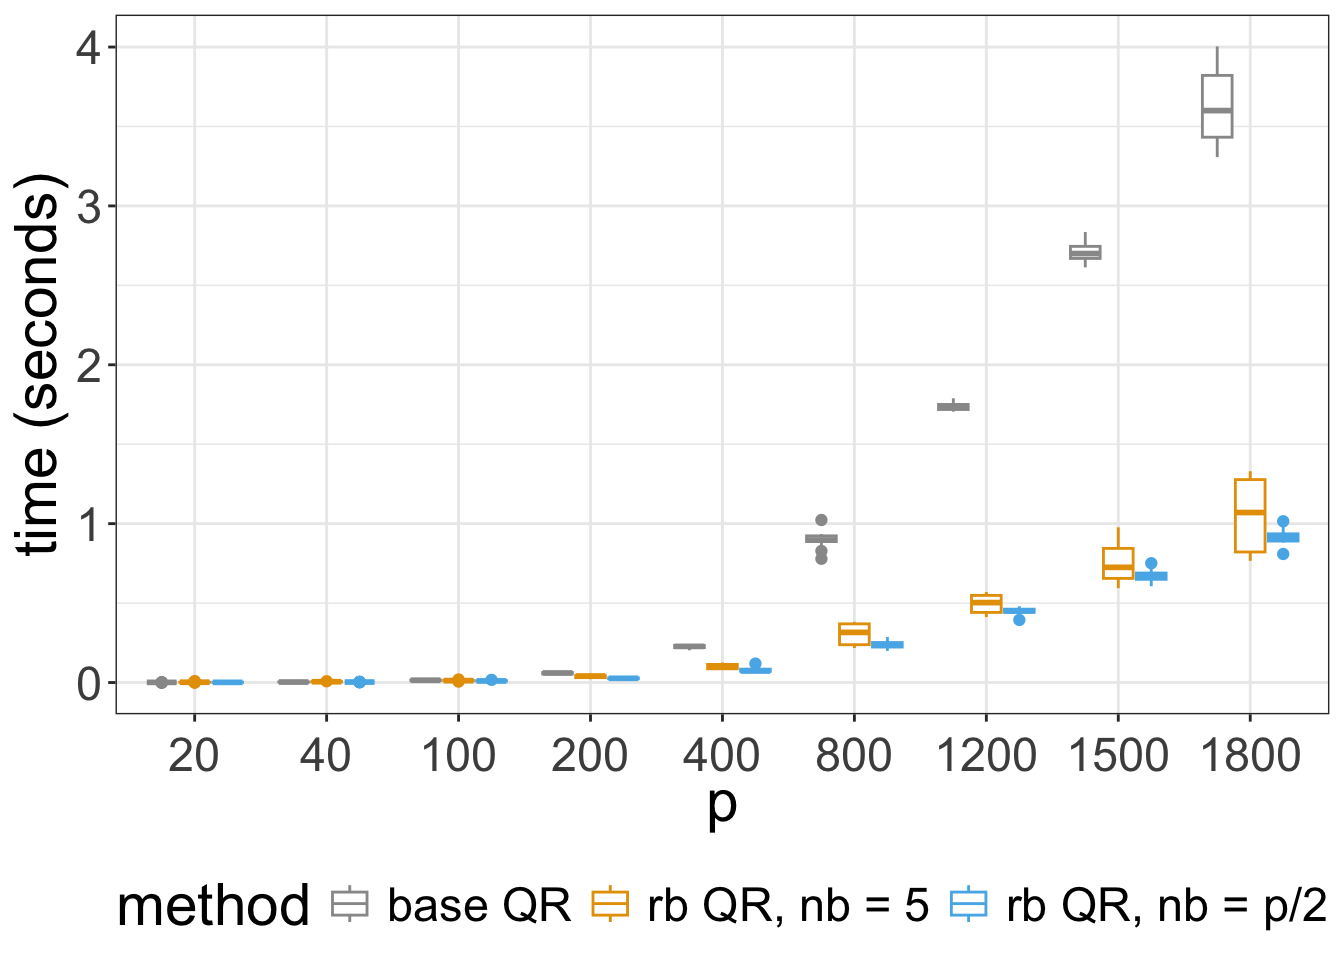
\includegraphics{fastQR_examples_files/figure-latex/unnamed-chunk-7-1}

\begin{Shaded}
\begin{Highlighting}[]
\NormalTok{width   }\OtherTok{\textless{}{-}} \DecValTok{10}
\NormalTok{height  }\OtherTok{\textless{}{-}}\NormalTok{ (}\DecValTok{9} \SpecialCharTok{/} \DecValTok{16}\NormalTok{) }\SpecialCharTok{*}\NormalTok{ width}
\NormalTok{fname   }\OtherTok{\textless{}{-}} \StringTok{"fastQR\_Chol\_decomposition\_comp\_time.pdf"}
\FunctionTok{ggsave}\NormalTok{(fname, }\AttributeTok{width =}\NormalTok{ width, }\AttributeTok{height =}\NormalTok{ height)}
\end{Highlighting}
\end{Shaded}

\hypertarget{solving-linear-systems}{%
\section{solving linear systems}\label{solving-linear-systems}}

\begin{Shaded}
\begin{Highlighting}[]
\CommentTok{\# Matrix dimensions to test}
\NormalTok{nrep }\OtherTok{\textless{}{-}} \DecValTok{10}
\NormalTok{n    }\OtherTok{\textless{}{-}} \DecValTok{1000}
\NormalTok{p    }\OtherTok{\textless{}{-}} \FunctionTok{c}\NormalTok{(}\DecValTok{20}\NormalTok{, }\DecValTok{40}\NormalTok{, }\DecValTok{60}\NormalTok{, }\DecValTok{80}\NormalTok{, }\DecValTok{100}\NormalTok{, }\DecValTok{120}\NormalTok{, }\DecValTok{140}\NormalTok{, }\DecValTok{160}\NormalTok{, }\DecValTok{180}\NormalTok{, }\DecValTok{200}\NormalTok{, }\DecValTok{300}\NormalTok{, }\DecValTok{500}\NormalTok{)}
\NormalTok{p}\SpecialCharTok{/}\DecValTok{4}
\end{Highlighting}
\end{Shaded}

\begin{verbatim}
##  [1]   5  10  15  20  25  30  35  40  45  50  75 125
\end{verbatim}

\begin{Shaded}
\begin{Highlighting}[]
\FunctionTok{detectCores}\NormalTok{()}
\end{Highlighting}
\end{Shaded}

\begin{verbatim}
## [1] 12
\end{verbatim}

\begin{Shaded}
\begin{Highlighting}[]
\NormalTok{ncores }\OtherTok{\textless{}{-}} \DecValTok{10}
\FunctionTok{registerDoParallel}\NormalTok{(}\AttributeTok{cores =}\NormalTok{ ncores)}

\CommentTok{\# time}
\NormalTok{output  }\OtherTok{\textless{}{-}} \ConstantTok{NULL}
\FunctionTok{set.seed}\NormalTok{(}\DecValTok{1234}\NormalTok{)}
\ControlFlowTok{for}\NormalTok{ (dim }\ControlFlowTok{in}\NormalTok{ p) \{}
\NormalTok{  results }\OtherTok{\textless{}{-}} \ConstantTok{NULL}
\NormalTok{  results }\OtherTok{\textless{}{-}}\NormalTok{ foreach}\SpecialCharTok{::}\FunctionTok{foreach}\NormalTok{(}\AttributeTok{rep =} \DecValTok{1}\SpecialCharTok{:}\NormalTok{nrep, }\AttributeTok{.packages =} \FunctionTok{c}\NormalTok{(}\StringTok{"fastQR"}\NormalTok{), }\AttributeTok{.combine =} \StringTok{"rbind"}\NormalTok{) }\SpecialCharTok{\%dopar\%}\NormalTok{ \{}
    \CommentTok{\#for (rep in 1:nrep) \{ }
    \CommentTok{\# print}
    \FunctionTok{cat}\NormalTok{(}\StringTok{"rep "}\NormalTok{, rep, }\StringTok{"}\SpecialCharTok{\textbackslash{}n}\StringTok{"}\NormalTok{)}
    
    \CommentTok{\# set seed}
    \CommentTok{\#set.seed(1234 + rep)}
    
    \CommentTok{\# Generate a random matrix}
\NormalTok{    y   }\OtherTok{\textless{}{-}} \FunctionTok{rnorm}\NormalTok{(n)}
\NormalTok{    X   }\OtherTok{\textless{}{-}} \FunctionTok{matrix}\NormalTok{(}\FunctionTok{rnorm}\NormalTok{(n }\SpecialCharTok{*}\NormalTok{ dim, }\DecValTok{1}\NormalTok{), n, dim)}
\NormalTok{    XTX }\OtherTok{\textless{}{-}} \FunctionTok{crossprod}\NormalTok{(X)}
\NormalTok{    XTy }\OtherTok{\textless{}{-}} \FunctionTok{crossprod}\NormalTok{(X, y)}
    
    \CommentTok{\# Measure fastQR, qr time}
\NormalTok{    qr\_time }\OtherTok{\textless{}{-}} \FunctionTok{system.time}\NormalTok{(fastQR}\SpecialCharTok{::}\FunctionTok{qrsolve}\NormalTok{(}\AttributeTok{A =}\NormalTok{ XTX, }\AttributeTok{b =}\NormalTok{ XTy, }\AttributeTok{nb =} \DecValTok{5}\NormalTok{))[}\StringTok{"elapsed"}\NormalTok{]}
\NormalTok{    res1    }\OtherTok{\textless{}{-}} \FunctionTok{data.frame}\NormalTok{(}\AttributeTok{p =}\NormalTok{ dim, }\AttributeTok{method =} \StringTok{"rb QR, nb = 5"}\NormalTok{, }\AttributeTok{time =}\NormalTok{ qr\_time)}
    
\NormalTok{    rbqr\_time }\OtherTok{\textless{}{-}} \FunctionTok{system.time}\NormalTok{(fastQR}\SpecialCharTok{::}\FunctionTok{qrsolve}\NormalTok{(}\AttributeTok{A =}\NormalTok{ XTX, }\AttributeTok{b =}\NormalTok{ XTy, }\AttributeTok{nb =}\NormalTok{ dim}\SpecialCharTok{/}\DecValTok{2}\NormalTok{))[}\StringTok{"elapsed"}\NormalTok{]}
\NormalTok{    res2      }\OtherTok{\textless{}{-}} \FunctionTok{data.frame}\NormalTok{(}\AttributeTok{p =}\NormalTok{ dim, }\AttributeTok{method =} \StringTok{"rb QR, nb = p/4"}\NormalTok{, }\AttributeTok{time =}\NormalTok{ rbqr\_time)}
    
    \CommentTok{\# Measure Solve time}
\NormalTok{    baseqr\_time }\OtherTok{\textless{}{-}} \FunctionTok{system.time}\NormalTok{(}\FunctionTok{qr.solve}\NormalTok{(}\FunctionTok{crossprod}\NormalTok{(X), }\FunctionTok{crossprod}\NormalTok{(X, y)))[}\StringTok{"elapsed"}\NormalTok{]}
\NormalTok{    res3        }\OtherTok{\textless{}{-}} \FunctionTok{data.frame}\NormalTok{(}\AttributeTok{p =}\NormalTok{ dim, }\AttributeTok{method =} \StringTok{"baseQR"}\NormalTok{,  }\AttributeTok{time =}\NormalTok{ baseqr\_time)}
    
    \CommentTok{\# return}
    \FunctionTok{rbind}\NormalTok{(results, }\FunctionTok{rbind}\NormalTok{(res1, res2, res3))}
\NormalTok{  \}}
\NormalTok{  output }\OtherTok{\textless{}{-}} \FunctionTok{rbind}\NormalTok{(output, results)}
\NormalTok{\}}
\FunctionTok{print}\NormalTok{(output }\SpecialCharTok{\%\textgreater{}\%}
        \FunctionTok{group\_by}\NormalTok{(p, method) }\SpecialCharTok{\%\textgreater{}\%}
        \FunctionTok{get\_summary\_stats}\NormalTok{(), }\AttributeTok{n =} \DecValTok{27}\NormalTok{)}
\end{Highlighting}
\end{Shaded}

\begin{verbatim}
## # A tibble: 36 x 15
##        p method  variable     n   min   max median    q1    q3   iqr   mad  mean
##    <dbl> <chr>   <fct>    <dbl> <dbl> <dbl>  <dbl> <dbl> <dbl> <dbl> <dbl> <dbl>
##  1    20 baseQR  time        10 0     0.001  0.001 0.001 0.001 0     0     0.001
##  2    20 rb QR,~ time        10 0     0.001  0     0     0.001 0.001 0.001 0    
##  3    20 rb QR,~ time        10 0     0      0     0     0     0     0     0    
##  4    40 baseQR  time        10 0.001 0.002  0.001 0.001 0.002 0.001 0     0.001
##  5    40 rb QR,~ time        10 0     0.001  0     0     0.001 0.001 0     0    
##  6    40 rb QR,~ time        10 0     0.001  0     0     0.001 0.001 0     0    
##  7    60 baseQR  time        10 0.002 0.003  0.003 0.002 0.003 0.001 0     0.003
##  8    60 rb QR,~ time        10 0     0.001  0.001 0.001 0.001 0     0     0.001
##  9    60 rb QR,~ time        10 0     0.001  0     0     0.001 0.001 0     0    
## 10    80 baseQR  time        10 0.004 0.006  0.005 0.004 0.005 0.001 0.001 0.005
## 11    80 rb QR,~ time        10 0     0.002  0.001 0     0.001 0.001 0     0.001
## 12    80 rb QR,~ time        10 0     0.001  0     0     0.001 0.001 0.001 0    
## 13   100 baseQR  time        10 0.005 0.008  0.006 0.006 0.007 0.001 0     0.006
## 14   100 rb QR,~ time        10 0     0.002  0.001 0.001 0.001 0     0     0.001
## 15   100 rb QR,~ time        10 0     0.001  0     0     0.001 0.001 0     0    
## 16   120 baseQR  time        10 0.008 0.009  0.009 0.008 0.009 0.001 0     0.009
## 17   120 rb QR,~ time        10 0.001 0.003  0.001 0.001 0.001 0     0     0.001
## 18   120 rb QR,~ time        10 0     0.002  0.001 0.001 0.002 0.001 0.001 0.001
## 19   140 baseQR  time        10 0.012 0.017  0.012 0.012 0.014 0.002 0     0.013
## 20   140 rb QR,~ time        10 0.001 0.003  0.002 0.002 0.003 0.001 0.001 0.002
## 21   140 rb QR,~ time        10 0.001 0.003  0.002 0.001 0.002 0.001 0.001 0.002
## 22   160 baseQR  time        10 0.015 0.022  0.018 0.016 0.021 0.005 0.003 0.018
## 23   160 rb QR,~ time        10 0.002 0.004  0.003 0.002 0.003 0.001 0.001 0.003
## 24   160 rb QR,~ time        10 0.001 0.005  0.002 0.002 0.003 0.001 0.001 0.003
## 25   180 baseQR  time        10 0.021 0.03   0.023 0.021 0.027 0.006 0.004 0.024
## 26   180 rb QR,~ time        10 0.002 0.006  0.003 0.002 0.004 0.002 0.001 0.003
## 27   180 rb QR,~ time        10 0.002 0.004  0.002 0.002 0.003 0.001 0     0.003
## # i 9 more rows
## # i 3 more variables: sd <dbl>, se <dbl>, ci <dbl>
\end{verbatim}

\begin{Shaded}
\begin{Highlighting}[]
\CommentTok{\# Convert factors to appropriate types}
\NormalTok{output}\SpecialCharTok{$}\NormalTok{p }\OtherTok{\textless{}{-}} \FunctionTok{as.factor}\NormalTok{(output}\SpecialCharTok{$}\NormalTok{p)}

\CommentTok{\# Plot the results}
\NormalTok{boxplot }\OtherTok{\textless{}{-}} \FunctionTok{ggplot}\NormalTok{(output, }\FunctionTok{aes}\NormalTok{(}\AttributeTok{x =}\NormalTok{ p, }\AttributeTok{y =}\NormalTok{ time)) }\SpecialCharTok{+}
  \FunctionTok{geom\_boxplot}\NormalTok{(}\FunctionTok{aes}\NormalTok{(}\AttributeTok{color =}\NormalTok{ method)) }\SpecialCharTok{+}
  \FunctionTok{labs}\NormalTok{(}
    \AttributeTok{x =} \StringTok{"p"}\NormalTok{,}
    \AttributeTok{y =} \StringTok{"time (seconds)"}\NormalTok{,}
    \AttributeTok{fill =} \StringTok{"method"}
\NormalTok{  ) }\SpecialCharTok{+}
  \FunctionTok{theme\_bw}\NormalTok{() }\SpecialCharTok{+}  
  \FunctionTok{theme}\NormalTok{(}\AttributeTok{text =} \FunctionTok{element\_text}\NormalTok{(}\AttributeTok{size =} \DecValTok{22}\NormalTok{)) }\SpecialCharTok{+}
  \FunctionTok{theme}\NormalTok{(}\AttributeTok{axis.text.x =} \FunctionTok{element\_text}\NormalTok{(}\AttributeTok{angle =} \DecValTok{0}\NormalTok{, }\AttributeTok{vjust =} \FloatTok{0.0}\NormalTok{, }\AttributeTok{hjust =}\NormalTok{ .}\DecValTok{50}\NormalTok{)) }\SpecialCharTok{+}
  \FunctionTok{theme}\NormalTok{(}
    \AttributeTok{legend.background    =} \FunctionTok{element\_rect}\NormalTok{(}\AttributeTok{fill =} \StringTok{"white"}\NormalTok{, }\AttributeTok{linewidth =} \DecValTok{4}\NormalTok{, }\AttributeTok{colour =} \StringTok{"white"}\NormalTok{),}
    \AttributeTok{legend.justification =} \StringTok{"center"}\NormalTok{,}
    \AttributeTok{legend.position      =} \StringTok{"bottom"}
\NormalTok{  ) }\SpecialCharTok{+}
  \CommentTok{\#ylim(c(0, 0.01)) +}
  \FunctionTok{scale\_color\_manual}\NormalTok{(}\AttributeTok{labels =} \FunctionTok{c}\NormalTok{(}\StringTok{"base QR"}\NormalTok{, }\StringTok{"rb QR, nb = 5"}\NormalTok{, }\StringTok{"rb QR, nb = p/2"}\NormalTok{), }\AttributeTok{values =}\NormalTok{ col\_pal) }\SpecialCharTok{+}
  \FunctionTok{guides}\NormalTok{(}\AttributeTok{fill =} \FunctionTok{guide\_legend}\NormalTok{(}\StringTok{"Method"}\NormalTok{)) }

\CommentTok{\# Display the boxplot}
\FunctionTok{print}\NormalTok{(boxplot)}
\end{Highlighting}
\end{Shaded}

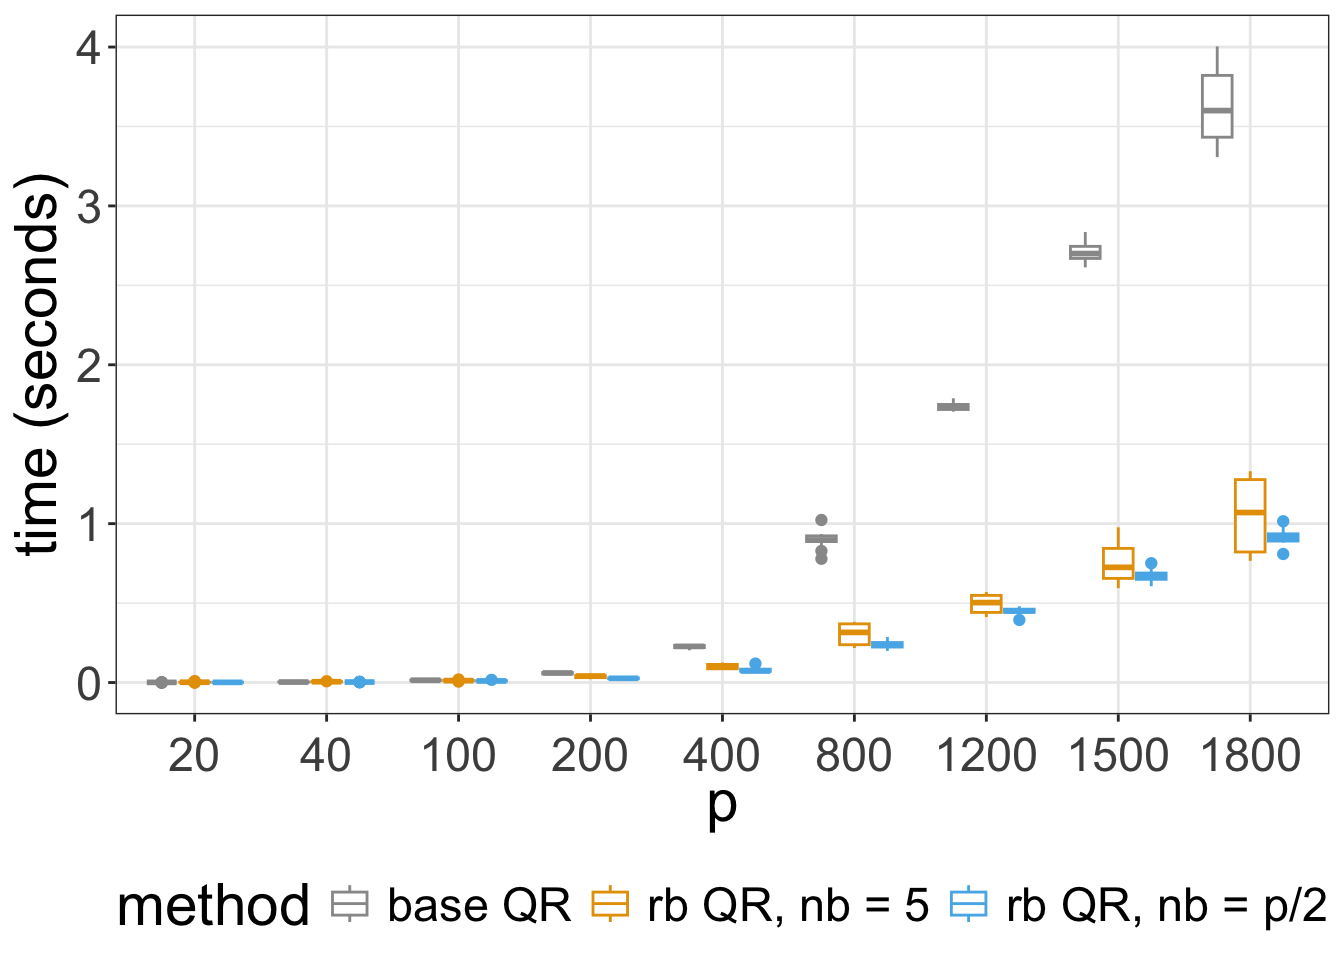
\includegraphics{fastQR_examples_files/figure-latex/unnamed-chunk-8-1}

\begin{Shaded}
\begin{Highlighting}[]
\NormalTok{width   }\OtherTok{\textless{}{-}} \DecValTok{10}
\NormalTok{height  }\OtherTok{\textless{}{-}}\NormalTok{ (}\DecValTok{9} \SpecialCharTok{/} \DecValTok{16}\NormalTok{) }\SpecialCharTok{*}\NormalTok{ width}
\NormalTok{fname   }\OtherTok{\textless{}{-}} \StringTok{"fastQR\_solve\_decomposition\_comp\_time.pdf"}
\FunctionTok{ggsave}\NormalTok{(fname, }\AttributeTok{width =}\NormalTok{ width, }\AttributeTok{height =}\NormalTok{ height)}
\end{Highlighting}
\end{Shaded}


\bibliography{skeleton.bib}



\end{document}
